%package list
\documentclass{article}
\usepackage[top=3cm, bottom=3cm, outer=3cm, inner=3cm]{geometry}
\usepackage{multicol}
\usepackage{graphicx}
\usepackage{url}
%\usepackage{cite}
\usepackage{hyperref}
\usepackage{array}
%\usepackage{multicol}
\newcolumntype{x}[1]{>{\centering\arraybackslash\hspace{0pt}}p{#1}}
\usepackage{natbib}
\usepackage{pdfpages}
\usepackage{multirow}
\usepackage[normalem]{ulem}
\useunder{\uline}{\ul}{}
\usepackage{svg}
\usepackage{xcolor}
\usepackage{listings}
\lstdefinestyle{ascii-tree}{
    literate={├}{|}1 {─}{--}1 {└}{+}1 
  }
\lstset{basicstyle=\ttfamily,
  showstringspaces=false,
  commentstyle=\color{red},
  keywordstyle=\color{blue}
}
%\usepackage{booktabs}
\usepackage{caption}
\usepackage{subcaption}
\usepackage{float}
\usepackage{array}

\newcolumntype{M}[1]{>{\centering\arraybackslash}m{#1}}
\newcolumntype{N}{@{}m{0pt}@{}}


%%%%%%%%%%%%%%%%%%%%%%%%%%%%%%%%%%%%%%%%%%%%%%%%%%%%%%%%%%%%%%%%%%%%%%%%%%%%
%%%%%%%%%%%%%%%%%%%%%%%%%%%%%%%%%%%%%%%%%%%%%%%%%%%%%%%%%%%%%%%%%%%%%%%%%%%%
\newcommand{\itemEmail}{jescobedooc@unsa.edu.pe}
\newcommand{\itemStudent}{Jorge Luis Escobedo Ocaña}
\newcommand{\itemCourse}{Programación Web 2}
\newcommand{\itemCourseCode}{20231001}
\newcommand{\itemSemester}{III}
\newcommand{\itemUniversity}{Universidad Nacional de San Agustín de Arequipa}
\newcommand{\itemFaculty}{Facultad de Ingeniería de Producción y Servicios}
\newcommand{\itemDepartment}{Departamento Académico de Ingeniería de Sistemas e Informática}
\newcommand{\itemSchool}{Escuela Profesional de Ingeniería de Sistemas}
\newcommand{\itemAcademic}{2023 - A}
\newcommand{\itemInput}{Del 25 Mayo 2023}
\newcommand{\itemOutput}{Al 08 Junio 2023}
\newcommand{\itemPracticeNumber}{04}
\newcommand{\itemTheme}{Python}
%%%%%%%%%%%%%%%%%%%%%%%%%%%%%%%%%%%%%%%%%%%%%%%%%%%%%%%%%%%%%%%%%%%%%%%%%%%%
%%%%%%%%%%%%%%%%%%%%%%%%%%%%%%%%%%%%%%%%%%%%%%%%%%%%%%%%%%%%%%%%%%%%%%%%%%%%

\usepackage[english,spanish]{babel}
\usepackage[utf8]{inputenc}
\AtBeginDocument{\selectlanguage{spanish}}
\renewcommand{\figurename}{Figura}
\renewcommand{\refname}{Referencias}
\renewcommand{\tablename}{Tabla} %esto no funciona cuando se usa babel
\AtBeginDocument{%
	\renewcommand\tablename{Tabla}
}

\usepackage{fancyhdr}
\pagestyle{fancy}
\fancyhf{}
\setlength{\headheight}{30pt}
\renewcommand{\headrulewidth}{1pt}
\renewcommand{\footrulewidth}{1pt}
\fancyhead[L]{\raisebox{-0.2\height}{
\includegraphics[width=3cm]{img/logo_episunsa.png}}}
\fancyhead[C]{\fontsize{7}{7}\selectfont	\itemUniversity \\ \itemFaculty \\ \itemDepartment \\ \itemSchool \\ \textbf{\itemCourse}}
\fancyhead[R]{\raisebox{-0.2\height}{\includegraphics[width=1.2cm]{img/logo_abet}}}
\fancyfoot[L]{Estudiante Jorge Escobedo Ocaña}
\fancyfoot[C]{\itemCourse}
\fancyfoot[R]{Página \thepage}

% para el codigo fuente
\usepackage{listings}
\usepackage{color, colortbl}
\definecolor{dkgreen}{rgb}{0,0.6,0}
\definecolor{gray}{rgb}{0.5,0.5,0.5}
\definecolor{mauve}{rgb}{0.58,0,0.82}
\definecolor{codebackground}{rgb}{0.95, 0.95, 0.92}
\definecolor{tablebackground}{rgb}{0.8, 0, 0}

\lstset{frame=tb,
	language=bash,
	aboveskip=3mm,
	belowskip=3mm,
	showstringspaces=false,
	columns=flexible,
	basicstyle={\small\ttfamily},
	numbers=none,
	numberstyle=\tiny\color{gray},
	keywordstyle=\color{blue},
	commentstyle=\color{dkgreen},
	stringstyle=\color{mauve},
	breaklines=true,
	breakatwhitespace=true,
	tabsize=3,
	backgroundcolor= \color{codebackground},
}

\begin{document}
	
	\vspace*{10px}
	
	\begin{center}	
		\fontsize{17}{17} \textbf{ Informe de Laboratorio \itemPracticeNumber}
	\end{center}
	\centerline{\textbf{\Large Tema: \itemTheme}}
	%\vspace*{0.5cm}	

	\begin{flushright}
		\begin{tabular}{|M{2.5cm}|N|}
			\hline 
			\rowcolor{tablebackground}
			\color{white} \textbf{Nota}  \\
			\hline 
			     \\[30pt]
			\hline 			
		\end{tabular}
	\end{flushright}	

	\begin{table}[H]
		\begin{tabular}{|x{4.7cm}|x{4.8cm}|x{4.8cm}|}
			\hline 
			\rowcolor{tablebackground}
			\color{white} \textbf{Estudiante} & \color{white}\textbf{Escuela}  & \color{white}\textbf{Asignatura}   \\
			\hline 
			{\itemStudent \par \itemEmail} & \itemSchool & {\itemCourse \par Semestre: \itemSemester \par Código: \itemCourseCode}     \\
			\hline 			
		\end{tabular}
	\end{table}		
	
	\begin{table}[H]
		\begin{tabular}{|x{4.7cm}|x{4.8cm}|x{4.8cm}|}
			\hline 
			\rowcolor{tablebackground}
			\color{white}\textbf{Laboratorio} & \color{white}\textbf{Tema}  & \color{white}\textbf{Duración}   \\
			\hline 
			\itemPracticeNumber & \itemTheme & 04 horas   \\
			\hline 
		\end{tabular}
	\end{table}
	
	\begin{table}[H]
		\begin{tabular}{|x{4.7cm}|x{4.8cm}|x{4.8cm}|}
			\hline 
			\rowcolor{tablebackground}
			\color{white}\textbf{Semestre académico} & \color{white}\textbf{Fecha de inicio}  & \color{white}\textbf{Fecha de entrega}   \\
			\hline 
			\itemAcademic & \itemInput &  \itemOutput  \\
			\hline 
		\end{tabular}
	\end{table}
	
	\section{Tarea}
    Implementar la clase Picture contará además con varios métodos:
	\begin{itemize}	
		\item verticalMirror: Devuelve el espejo vertical de la imagen
		\item horizontalMirror: Devuelve el espejo horizontal de la imagen
        \item negative: Devuelve un negativo de la imagen
        \item join: Devuelve una nueva figura poniendo la figura del argumento al lado derecho de la figura actual
        \item up: Devuelve una nueva figura poniendo la figura recibida como argumento, encima de la figura actual
        \item under: Devuelve una nueva figura poniendo la figura recibida como argumento, sobre la figura actual
        \item horizontalRepeat, Devuelve una nueva figura repitiendo la figura actual al costado la cantidad de veces que indique el valor de n
        \item verticalRepeat Devuelve una nueva figura repitiendo la figura actual debajo, la cantidad de veces que indique el valor de n
	\end{itemize}
		
	\section{Equipos, materiales y temas utilizados}
	\begin{itemize}
		\item Sistema Operativo Ubuntu GNU Linux 23 lunar 64 bits Kernell 6.2.
		\item VIM 9.0.
		\item Python 3.
		\item Git 2.39.2.
		\item Cuenta en GitHub con el correo institucional.
		\item Programación Orientada a Objetos.	
	\end{itemize}
	
	\section{URL de Repositorio Github}
	\begin{itemize}
		\item URL del Repositorio GitHub para clonar o recuperar.
		\item \url{https://github.com/Juerges28/Lab04-Pweb2.git}
		\item URL para el laboratorio 04 en el Repositorio GitHub.
		\item \url{https://github.com/rescobedoq/programacion/tree/main/lab04}
	\end{itemize}
	
	\section{Actividades con el repositorio GitHub}
	
	\subsection{Creando e inicializando repositorio GitHub}
	\begin{itemize}	
		\item Como es el primer laboratorio se creo el repositorio GitHub.
		\item Se realizaron los siguientes comandos en la computadora:
	\end{itemize}	
		
	\begin{lstlisting}[language=bash,caption={Creando directorio de trabajo}][H]
		$ mkdir -p Lab04-Pweb2/
	\end{lstlisting}
	\begin{lstlisting}[language=bash,caption={Dirijíéndonos al directorio de trabajo}][H]
		$ cd Lab04-Pweb2/
	\end{lstlisting}	
	\begin{lstlisting}[language=bash,caption={Creando directorio para repositorio GitHub}][H]
		$ mkdir -p Lab04-Pweb2/
	\end{lstlisting}
	\begin{lstlisting}[language=bash,caption={Inicializando directorio para repositorio GitHub}][H]
		$ cd Lab04-Pweb2/
		$ echo "# programacion" >> README.md
		$ git init
		$ git config --global user.name "Jorge Luis Escobedo Ocaña"
		$ git config --global user.email jescobedooc@unsa.edu.pe
		$ git add README.md
		$ git commit -m "first commit"
		$ git branch -M main
		$ git remote add origin https://github.com/Juerges28/Lab04-Pweb2.git
		$ git push -u origin main
	\end{lstlisting}
	
	\subsection{Commits}
	\begin{lstlisting}[language=bash,caption={Primer Commit Creando carpeta/archivo para laboratorio 01}][H]
        $ mkdir Tarea-del-Ajedrez/
        $ touch Tarea-del-Ajedrez/pieces.py
        $ touch Tarea-del-Ajedrez/picture.py
        $ touch Tarea-del-Ajedrez/colors.py
        $ touch Tarea-del-Ajedrez/chessPictures.py
        $ git add .
        $ git commit -m "Creando Tarea-del-Ajedrez/archivos para laboratorio 04"			
        $ git push -u origin main
	\end{lstlisting}
	
	\begin{itemize}	
		\item Para el siguiente commit se implementaron los metodos en la clase picture.py necesarios para realizar los ejercicios.
	\end{itemize}	

    \begin{figure}[htbp]
        \begin{minipage}{0.5\textwidth}
            \centering
            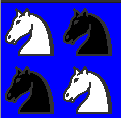
\includegraphics[width=0.5\linewidth]{img/ejercicio_02_a.png}
            \caption{Ejercicio 2a}
            \label{fig:1l}
        \end{minipage}%
        \begin{minipage}{0.5\textwidth}
            \centering
            
\includegraphics[width=0.5\linewidth]{img/ejercicio_02_b.png}
            \caption{Ejercicio 2b}
            \label{fig:2}
        \end{minipage}
    \end{figure}
 \begin{figure}[htbp]
        \begin{minipage}{0.5\textwidth}
            \centering
            
\includegraphics[width=0.75\linewidth]{img/ejercicio_02_c.png}
            \caption{Ejercicio 2c}
            \label{fig:3}
        \end{minipage}%
        \begin{minipage}{0.5\textwidth}
            \centering
            
\includegraphics[width=0.75\linewidth]{img/ejercicio_02_d.png}
            \caption{Ejercicio 2d}
            \label{fig:4}
        \end{minipage}
    \end{figure}
    \begin{figure}[htbp]
        \begin{minipage}{0.5\textwidth}
            \centering
            
\includegraphics[width=0.75\linewidth]{img/ejercicio_02_e.png}
            \caption{Ejercicio 2e}
            \label{fig:5}
        \end{minipage}%
        \begin{minipage}{0.5\textwidth}
            \centering
            
\includegraphics[width=0.75\linewidth]{img/ejercicio_02_f.png}
            \caption{Ejercicio 2f}
            \label{fig:6}
        \end{minipage}
    \end{figure}
	\clearpage
	\begin{figure}
	    \centering
	    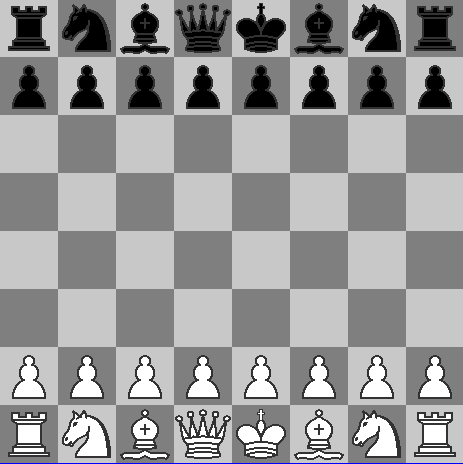
\includegraphics[width=0.5\linewidth]{img/ejercicio_02_g.png}
	    \caption{Ejercicio 2g}
	    \label{fig:7}
	\end{figure}
\begin{itemize}
    \item Implementamos los metodos necesarios en la clase picture.py para el desarrollo en los ejercicios.
\end{itemize}

 \begin{lstlisting}[language=bash,caption={Modificando picture.py}][H]
		$ vim Tarea-del-Ajedrez/picture.py
	\end{lstlisting}
	
	\lstinputlisting[language=python, caption={picture.py},numbers=left,]{src/picture.py}
\clearpage
	\begin{lstlisting}[language=bash,caption={Commit: Guardando cambios en picture.py}][H]
		$ git add .
		$ git commit -m "Guardando cambios en picture.py"			
		$ git push -u origin main
	\end{lstlisting}
 
 \begin{lstlisting}[language=bash,caption={Creando Ejercicio2a.py}][H]
		$ vim Tarea-del-Ajedrez/Ejercicio2a.py
	\end{lstlisting}
	
	\lstinputlisting[language=python, caption={Ejercicio2a.py},numbers=left,]{src/Ejercicio2a.py}
\begin{itemize}
    \item  Se comprueba la igualdad a la imagen planteada como ejercicio.
\end{itemize}

	\begin{lstlisting}[language=bash,caption={Probando código}][H]
		$ cd Tarea-del-Ajedrez
		$ python Ejercicio2a.py
	\end{lstlisting}
 
	\begin{lstlisting}[language=bash,caption={Commit: Comprobacion de exito del Ejercicio 2a}][H]
		$ git add .
		$ git commit -m "Comprobacion de exito del Ejercicio 2a"			
		$ git push -u origin main
	\end{lstlisting}

\begin{lstlisting}[language=bash,caption={Creando Ejercicio2b.py}][H]
		$ vim Tarea-del-Ajedrez/Ejercicio2b.py
	\end{lstlisting}
	
	\lstinputlisting[language=python, caption={Ejercicio2b.py},numbers=left,]{src/Ejercicio2b.py}
\begin{itemize}
    \item  Se comprueba la igualdad a la imagen planteada como ejercicio.
\end{itemize}

	\begin{lstlisting}[language=bash,caption={Probando código}][H]
		$ cd Tarea-del-Ajedrez
		$ python Ejercicio2b.py
	\end{lstlisting}
	\begin{lstlisting}[language=bash,caption={Commit: Comprobacion de exito del Ejercicio 2b}][H]
		$ git add .
		$ git commit -m "Comprobacion de exito del Ejercicio 2b"			
		$ git push -u origin main
	\end{lstlisting}
 
		 \begin{lstlisting}[language=bash,caption={Creando Ejercicio2c.py}][H]
		$ vim Tarea-del-Ajedrez/Ejercicio2c.py
	\end{lstlisting}
	
	\lstinputlisting[language=python, caption={Ejercicio2c.py},numbers=left,]{src/Ejercicio2c.py}
\begin{itemize}
    \item  Se comprueba la igualdad a la imagen planteada como ejercicio.
\end{itemize}

	\begin{lstlisting}[language=bash,caption={Probando código}][H]
		$ cd Tarea-del-Ajedrez
		$ python Ejercicio2c.py
	\end{lstlisting}
	\begin{lstlisting}[language=bash,caption={Commit: Comprobacion de exito del Ejercicio 2c}][H]
		$ git add .
		$ git commit -m "Comprobacion de exito del Ejercicio 2c"			
		$ git push -u origin main
	\end{lstlisting}

 \begin{lstlisting}[language=bash,caption={Creando Ejercicio2d.py}][H]
		$ vim Tarea-del-Ajedrez/Ejercicio2d.py
	\end{lstlisting}
	
	\lstinputlisting[language=python, caption={Ejercicio2d.py},numbers=left,]{src/Ejercicio2d.py}
\begin{itemize}
    \item  Se comprueba la igualdad a la imagen planteada como ejercicio.
\end{itemize}

	\begin{lstlisting}[language=bash,caption={Probando código}][H]
		$ cd Tarea-del-Ajedrez
		$ python Ejercicio2d.py
	\end{lstlisting}
	\begin{lstlisting}[language=bash,caption={Commit: Comprobacion de exito del Ejercicio 2d}][H]
		$ git add .
		$ git commit -m "Comprobacion de exito del Ejercicio 2d"			
		$ git push -u origin main
	\end{lstlisting}

 \begin{lstlisting}[language=bash,caption={Creando Ejercicio2e.py}][H]
		$ vim Tarea-del-Ajedrez/Ejercicio2e.py
	\end{lstlisting}
	
	\lstinputlisting[language=python, caption={Ejercicio2e.py},numbers=left,]{src/Ejercicio2e.py}
\begin{itemize}
    \item  Se comprueba la igualdad a la imagen planteada como ejercicio.
\end{itemize}

	\begin{lstlisting}[language=bash,caption={Probando código}][H]
		$ cd Tarea-del-Ajedrez
		$ python Ejercicio2e.py
	\end{lstlisting}
	\begin{lstlisting}[language=bash,caption={Commit: Comprobacion de exito del Ejercicio 2e}][H]
		$ git add .
		$ git commit -m "Comprobacion de exito del Ejercicio 2e"			
		$ git push -u origin main
	\end{lstlisting}
 
		 \begin{lstlisting}[language=bash,caption={Creando Ejercicio2f.py}][H]
		$ vim Tarea-del-Ajedrez/Ejercicio2f.py
	\end{lstlisting}
	
	\lstinputlisting[language=python, caption={Ejercicio2f.py},numbers=left,]{src/Ejercicio2f.py}
\begin{itemize}
    \item  Se comprueba la igualdad a la imagen planteada como ejercicio.
\end{itemize}

	\begin{lstlisting}[language=bash,caption={Probando código}][H]
		$ cd Tarea-del-Ajedrez
		$ python Ejercicio2f.py
	\end{lstlisting}
	\begin{lstlisting}[language=bash,caption={Commit: Comprobacion de exito del Ejercicio 2f}][H]
		$ git add .
		$ git commit -m "Comprobacion de exito del Ejercicio 2f"			
		$ git push -u origin main
	\end{lstlisting}

 \begin{lstlisting}[language=bash,caption={Creando Ejercicio2g.py}][H]
		$ vim Tarea-del-Ajedrez/Ejercicio2g.py
	\end{lstlisting}
	
	\lstinputlisting[language=python, caption={Ejercicio2g.py},numbers=left,]{src/Ejercicio2g.py}
\begin{itemize}
    \item  Se comprueba la igualdad a la imagen planteada como ejercicio.
\end{itemize}

	\begin{lstlisting}[language=bash,caption={Probando código}][H]
		$ cd Tarea-del-Ajedrez
		$ python Ejercicio2g.py
	\end{lstlisting}
	\begin{lstlisting}[language=bash,caption={Commit: Comprobacion de exito del Ejercicio 2g}][H]
		$ git add .
		$ git commit -m "Comprobacion de exito del Ejercicio 2g"			
		$ git push -u origin main
	\end{lstlisting}
	\subsection{Estructura de laboratorio 04}
	\begin{itemize}	
		\item El contenido que se entrega en este laboratorio es el siguiente:
	\end{itemize}
	
\begin{lstlisting}[style=ascii-tree]
Tarea-del-Ajedrez/
|--- Ejercicio2a.py
|--- Ejercicio2b.py
|--- Ejercicio2c.py
|--- Ejercicio2d.py
|--- Ejercicio2e.py
|--- Ejercicio2f.py
|--- Ejercicio2g.py
|--- chessPictures.py
|--- colors.py
|--- interpreter.py
|--- picture.py
|--- pieces.py
|--- latex
    |--- img
    |   |--- logo_abet.png
    |   |--- logo_episunsa.png
    |   |--- logo_unsa.jpg
    |   |--- pseudocodigo_insercion.png
    |   |--- ejercicio_02_a.png
    |   |--- ejercicio_02_b.png
    |   |--- ejercicio_02_c.png
    |   |--- ejercicio_02_d.png
    |   |--- ejercicio_02_e.png
    |   |--- ejercicio_02_f.png
    |   |--- ejercicio_02_g.png
    |--- pweb2_lab04_jescobedooc_v1.0.pdf    
    |--- pweb2_lab04_jescobedooc_v1.0.tex 
    |--- src
        |--- Ejercicio2a.py
        |--- Ejercicio2b.py
        |--- Ejercicio2c.py
        |--- Ejercicio2d.py
        |--- Ejercicio2e.py
        |--- Ejercicio2f.py
        |--- Ejercicio2g.py
        |--- picture.py
\end{lstlisting}    
\clearpage
\section{CUESTIONARIO}
	\begin{itemize}
		\item ¿Qué son los archivos *.pyc? \\
        Los archivos .pyc son archivos de código compilado generados por Python. Contienen el código fuente de un archivo .py que ha sido compilado en bytecode de Python. Los archivos .pyc permiten una ejecución más rápida del código, ya que evitan la necesidad de recompilar el archivo .py cada vez que se ejecuta.
  \item ¿Para qué sirve el directorio pycache?\\
        El directorio "pycache" se utiliza para almacenar los archivos .pyc generados por Python. Estos archivos se crean para mejorar el rendimiento al ejecutar el código Python, ya que evitan la necesidad de recompilar el código fuente cada vez que se ejecuta.        
  \item ¿Cuáles son los usos y lo que representa el subguión en Python?\\
        El subguión (\_) en Python tiene varios usos:\\
1. Como nombre de variable temporal o descartada cuando no es relevante.\\
2. En interpretadores interactivos, se utiliza para almacenar el resultado de la expresión anterior.\\
3. En convenciones de nomenclatura, puede indicar que una variable o método es de uso interno y no debe accederse directamente desde fuera de la clase o módulo.\\
En resumen, el subguión se utiliza para representar variables o elementos que no son relevantes o que tienen un uso específico en Python.
        
	\end{itemize}		
\clearpage

\section{Referencias}
\begin{itemize}			
	\item https://www.w3schools.com/python/python\_reference.asp
 \item https://docs.python.org/3/tutorial/
\end{itemize}	
	
%\clearpage
%\bibliographystyle{apalike}
%\bibliographystyle{IEEEtranN}
%\bibliography{bibliography}
			
\end{document}
